\documentclass[12pt]{article}
\usepackage{hyperref}
\usepackage{enumerate}
\usepackage{latexsym}
\usepackage{amssymb,amsmath}
\usepackage[pdftex]{graphicx}


\topmargin = 0.1in \textwidth=5.7in \textheight=8.6in

\oddsidemargin = 0.2in \evensidemargin = 0.2in


\begin{document}

\begin{center}
Applied Mathematics 115, FALL 2015 \\


Theresa Bischoff, Steven Petterutti, Tina Qian, Varun Sriram

\medskip

\textbf{ODE Modeling Age of Empires}


\end{center}

\begin{abstract}
	We modeled the game "Age of Empires," in which rival civilizations attempt to achieve world domination by destroying one another. Our goal is to consider different game strategies and to optimize conditions against enemy AI. By modeling the interaction between two civilizations with sets of ODEs for various strategies, and by performing stability/parameter analysis, we determined the necessary conditions for staying alive and ultimately, winning the game. We found that certain settings of aprameters can in fact doom us to lose, and solved for the settings of parameters and initial conditions that can help us win.
	
\end{abstract}

\section{Introduction}
\paragraph{}
In "Age of Empires," civilizations are pitted against one another, with the objective of winning the game by having the enemy surrender. Each cilization is limited to a certain population size by the game, a "carrying capacity" of typically $200$. Population is split between villagers and military, a designation decided at birth. Villagers gather resources that can be used for births - essentially, villagers can be thought of as the only ones "reproducing." In the game, reproducing can in theory happen infinitely, since structures such as Mills provide a source of infinite resources. Military units are harder to kill and are also the only ones that can attack and kill enemy units. Finally, note that natural births do not exist in the game - if no one is killed, no one dies. \par
In our analysis, we let civilization $C_1$ represent our civilization and civilization $C_2$ represent the enemy AI civilization. We let $C_1 = M_1 + V_1$ and $C_2 = M_2 + V_2$ where the $M_i$ and $V_i$ represent military and villager populations respectively for civilization $i$. The AI civilization surrenders when their numbers fall below a certain threshold $T$, or when our population stabilizes at some nonzero value (the enemy will never be able to kill all our units) - these are conditions for the AI to surrender embedded in the code for the game. \par
When initializing a game, setting certain parameters to specific values can maximize our chances of defeating the AI civilization - these include initial populations of the AI, AI intelligence level and military skills, new unit spawn speed, and map size. Furthermore, parameters such as how fast we click to destroy military units (that is parameter dictating our game performance) can also maximize or hurt our chances defeating the AI civilization. In this project, by exploring models of game strategy, considering phase diagrams, and exploring initial conditions/ parameter sensitivity, we gain insight into what we should set these parameters to, and thus what we can do to maximize our chances of winning. \par

\section{The Model}

\subsection{Scenario 1}

In our first scenario, $C_2$, the enemy AI civilization, starts off with only military. We, $C_1$, choose the strategy of only producing villagers, and not budgeting any reproductive resources to the military. This leads to a model similar to predator prey. \par

$M_1(0) = 0$, $V_1(0)$ and $M_2(0)$ are initial conditions we can vary when initializing the game, and $V_2(0) = 0$.

$$\dot V_1=\alpha V_1(1-\frac{V_1}{k})-V_1(\frac{M_2^2}{A^2+M_2^2})$$
$$ \dot M_i = 0 \text{ for } i \in \{1, 2\} $$
$$\dot V_2 = 0$$

Let us explain our reasoning for the equation for $\dot V_1$. The first term represents logistic growth, such that the carrying capacity is set at $k=200$ by the game code, and the reproduction rate $\alpha$ is determined by (1) what we set the military/villager spawn rate to when initializing the game and (2) how quickly we can click on villagers to gather resources, since the sooner we get more resources, the faster we can create a new villager. The second term represents the predation term where $V_1$ represents the limit that $M_2$ can kill (also ensures that $\dot V_1$ falls to 0 when $V_1 = 0$) and $A$ represents the point at which predation rapidly increases as it is easier to find and kill with more units. Note that $A$ will need to be larger with larger map sizes, and by setting the map size parameter when initializing a game, we effectively vary $A$. In this scenario, we have 2 parameters and 2 initial conditions that we may vary, and $\dot C_1 = \dot V_1$ while $\dot C_2 = 0$. We will investigate what initial conditions and parameter combinations will lead to our victory. In this case, we can win only by stabilizing at a nonzero population in the long run, since we have no military.


\subsection{Scenario 2}

In our second scenario, we initialize the game again so that the AI civilization $C_2$ starts off with only military. However, we, $C_1$, choose now to produce both military and villagers. It is now possible for us to win by either stabilizing our long-run population to be nonzero or wiping out the AI population to $T$. Without loss of generality, let $T = 0$. \par


$$\dot M_1=a \alpha V_1(1-\frac{V_1}{(1-a)K})-[M_1D_1(\frac{M_2^2}{A+M_2^2})(\frac{1}{A+M_1^2})]$$
$$\dot V_1=(1 - a) \alpha V_1(1-\frac{V_1}{(1-a)K})-[V_1cD_1(\frac{M_2^2}{A+M_2^2})(\frac{1}{A +M_1})]$$
$$\dot M_2=-M_2 D_2(\frac{M_1^2}{A+M_1^2})(\frac{1}{A +M_2^2}) $$
$$\dot V_2 = 0 $$

Let us explain our reasoning for this set of ODEs. For civilization 1, the first terms in $\dot M_1$ and $\dot V_1$ represent logistic growth. There is dependence only on $V_1$, since only villagers reproduce. Here the reproduction rate of military and of villagers are $a \alpha$ and $(1 - a) \alpha$ respectively where the $a$ now represents the fraction that we devote to military. The carrying capacity is $(1-a)K$ for villagers, which is what we care about in the equation. For civilization 1, the second term represents the predation term, which depends on both $M_1$ and $M_2$. It was derived by holding the other variable constant, considering how predation is affected by the variable in question, and then choosing the best functional form to represent this. The $M_1 (\frac{M_2^2}{A+M_2^2})$ and $V_1 (\frac{M_2^2}{A+M_2^2})$ terms represent how $M_2$ affects predation on $M_1$ and $V_1$ respectively, where the multiplication by $M_1$ and $V_1$ represent maximum kill limits. The $A$ again is controlled by map size, and represents the point at which predation becomes easier because you have enough $M_2$ to find enemy units. The $M_1 D_1 (\frac{1}{A+M_1^2})$ and the $D_1 (\frac{1}{A +M_1})$ represent the relationship between $M_1$ and predation. When $M_1$ is small, predation will rise, but when $M_1$ gets large enough (controlled by $A$), predation will fall. The $D_1$ is a parameter that controlls how effectively $C_2$ can kill $C_1$ military units, where larger values indicate they are more effective. $c = 6$ because military units have 6x the life points of villager units, and thus villagers are 6x easier to kill. For civlization 2, there is no growth because $V_2 = 0$ for all $t$. There is only a predation term on $M_2$ that is symmetricly formed; the parameter $D_2$ controlls how effectively we, $C_1$, can vanquish $M_2$. This is determined largely by our clicking speed in the game. \par
The number of parameters we can control in this system is 5 - we can control $A$ with map size, $D_1$ is controlled by AI speed and intelligence (which can be set at game initialization), $D_2$ is controlled by our clicking speed in the game, $a$ is the strategy of villager/military allocation we employ in the game, and $\alpha$ is reproduction rate overall which is controlled mostly by spawn rates we set at game initialization.

\subsection{Scenario 3}

 In our final scenario, $C_1$ produces both villagers and military units as before. However, we initialize $C_2$ to start with some villagers as well, and they produce both villagers and military units. Now, we write out equations for $C_2$ that are symmetric to the equations for $C_1$, following the same logic for our model as scenario 2: 

$$\dot M_1 =a_1 \alpha V_1(1-\frac{V_1}{(1 - a_1) K})-[M_1D_1(\frac{M_2^2}{A+M_2^2})(\frac{1}{A+M_1^2})]$$
$$\dot V_1=(1 - a_1) \alpha V_1(1-\frac{V_1}{(1 - a_1)K})-[V_1c D_1(\frac{M_2^2}{A+M_2^2})(\frac{1}{A +M_1})]$$
$$\dot M_2=a_2 \beta V_2(1-\frac{V_2}{(1 - a_2)K})-[M_2 D_2(\frac{M_1^2}{A+M_1^2})(\frac{1}{A +M_2^2})] $$
$$\dot V_2=(1 - a_2) \beta V_2(1-\frac{V_2}{(1-a_2)K})-[V_2 c D_2(\frac{M_1^2}{A+M_1^2})(\frac{1}{A +M_2})] $$

Here we have 6 parameters. The additional paramter is $\beta$ which is determined only by spawn rate of units. If we are as fast as the AI at clicking villagers to gather resources, then $\alpha = \beta$. Note that $a_2$ isn't really a parameter, since the military/villager allocation is set in the game code. Proportional allocation as we have here is a bit of a simplification of the allocation schedule, but we will let $a_2 = 0.5$.

\section{Analysis of the Model}

\subsection{Scenario 1}

Because we only have one nontrivial ODE, we can perform algebraic analysis more easily. Let us consider the fixed points of the system. $V_1 = 0$ is trivially a fixed point, because if $V_1 = 0$, the system is stuck at $M_2 = M_2(0)$ since $C_1$ cannot reproduce. If $V_1$ starts off with a non-zero value, then we have a more interesting dependence on paramenters $A$ and $\alpha$ as well as initial condition $M_2(0)$. By setting $\dot V_1$ to 0, and dividing out the $V_1$, since we are only considering fixed points where $V_1 > 0$ now, we get $V_1 = k(1 - \frac{1}{\alpha} \frac{M_2^2}{A^2 + M_2^2})$ as the fixed point. Note though that because $V_1 > 0$, this requires that $\frac{1}{\alpha} \frac{M_2^2}{A^2 + M_2^2} < 1$. Rearranging, the requirement for a non-zero $V_1$ fixed point existence is $M_2^2 < \frac{\alpha}{1 - \alpha} A^2$.\par
In the following phase portrait, we set $\alpha = 0.5$ indicating a reasonable spawn rate, and $A=10$ indicating a rather small map. According to our above analysis, we will need $M_2^2 < 100$ meaning that when $M_2(0) < 10$, we will have a stable fixed point at nonzero $V_1$ implying that we win the game. Otherwise, we are doomed to lose the game. This is also clearly illustrated in our phase portrait where the red dots indicate fixed points. The red dots are at nonzero $C_1 = V_1$ when $M_2 < 10$. The arrows also illustrate that these are stable fixed points.  Here is a picture of the phase diagram that produced these results (from Code Snippet 1):
\begin{center}
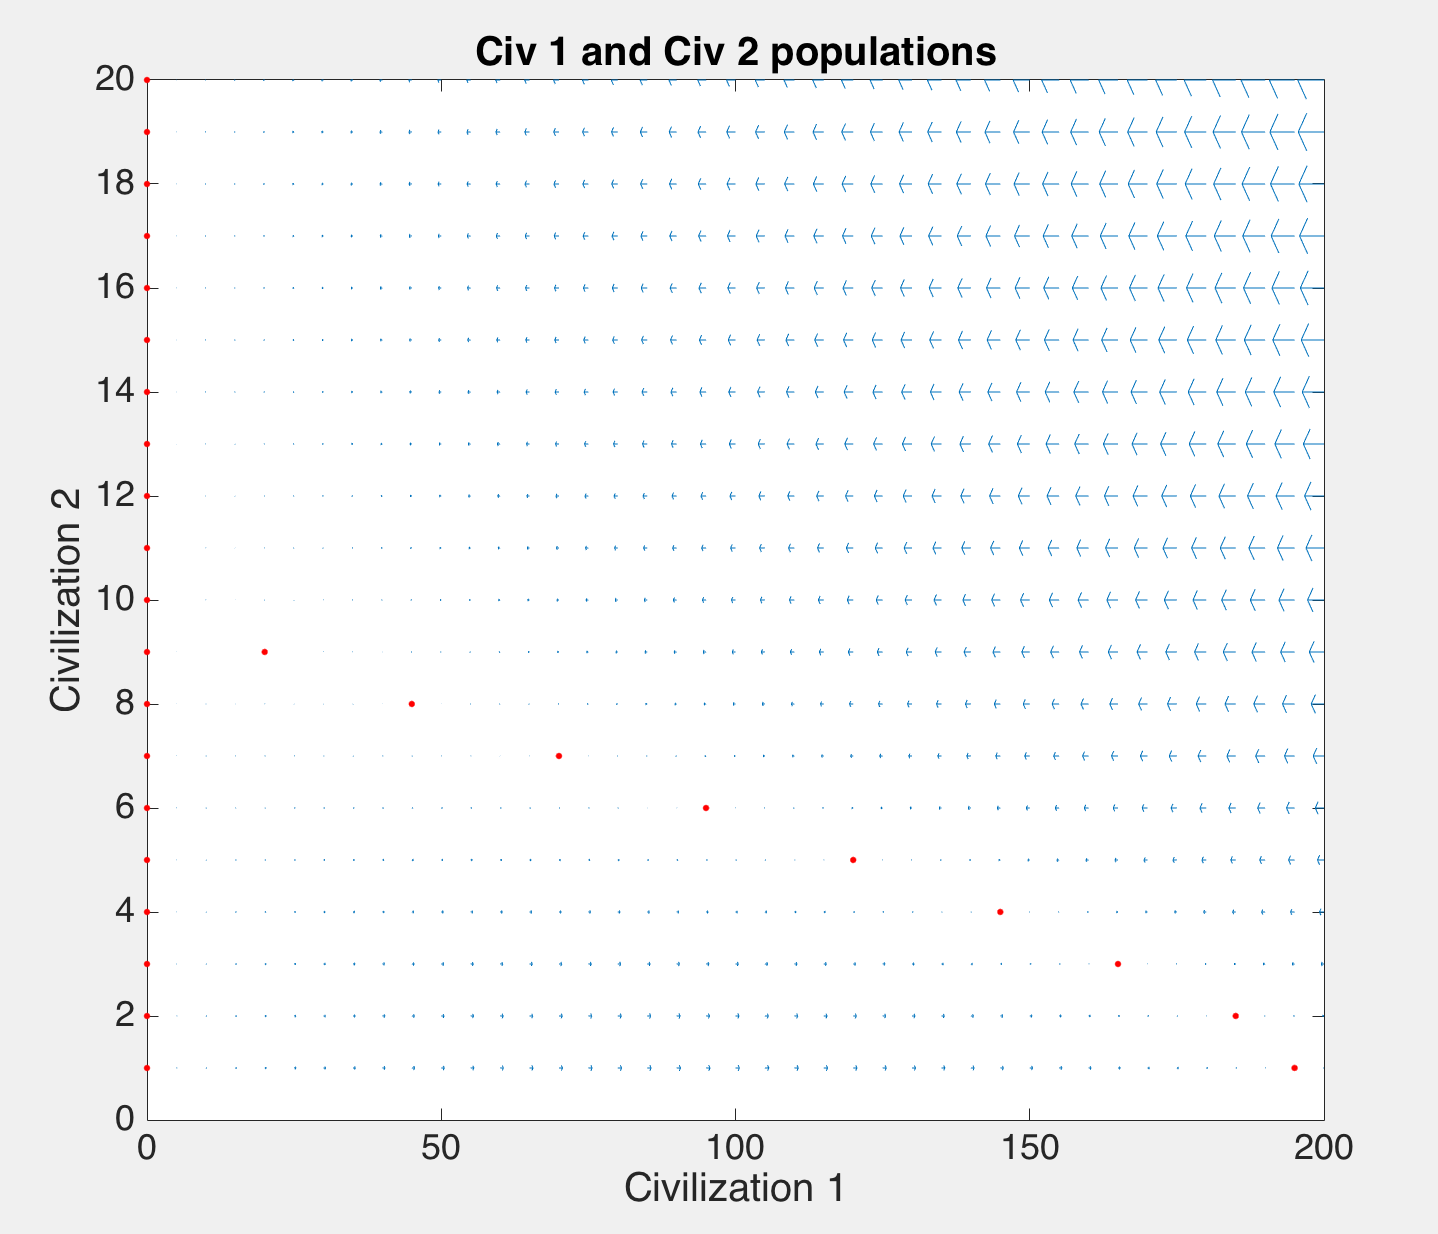
\includegraphics[width=250pt]{phaseplot_basic}
\end{center}

Below is a contour plot (from Code Snippet 2) illustrating how the fixed point $V_1$ varies with the parameters $A$ and $\alpha$. We let $M_2(0) = 200$, and $V_1(0) = 50$. Specifically, since $A < 200$, $\alpha > 0.5$ for us to win. As you can see, this is justified by the contour plot. Also, for fixed A, higher alpha means our population stabilizes at a higher value, and likewise, for fixed alpha, higher A means a higher stable $V_1$:
\begin{center}
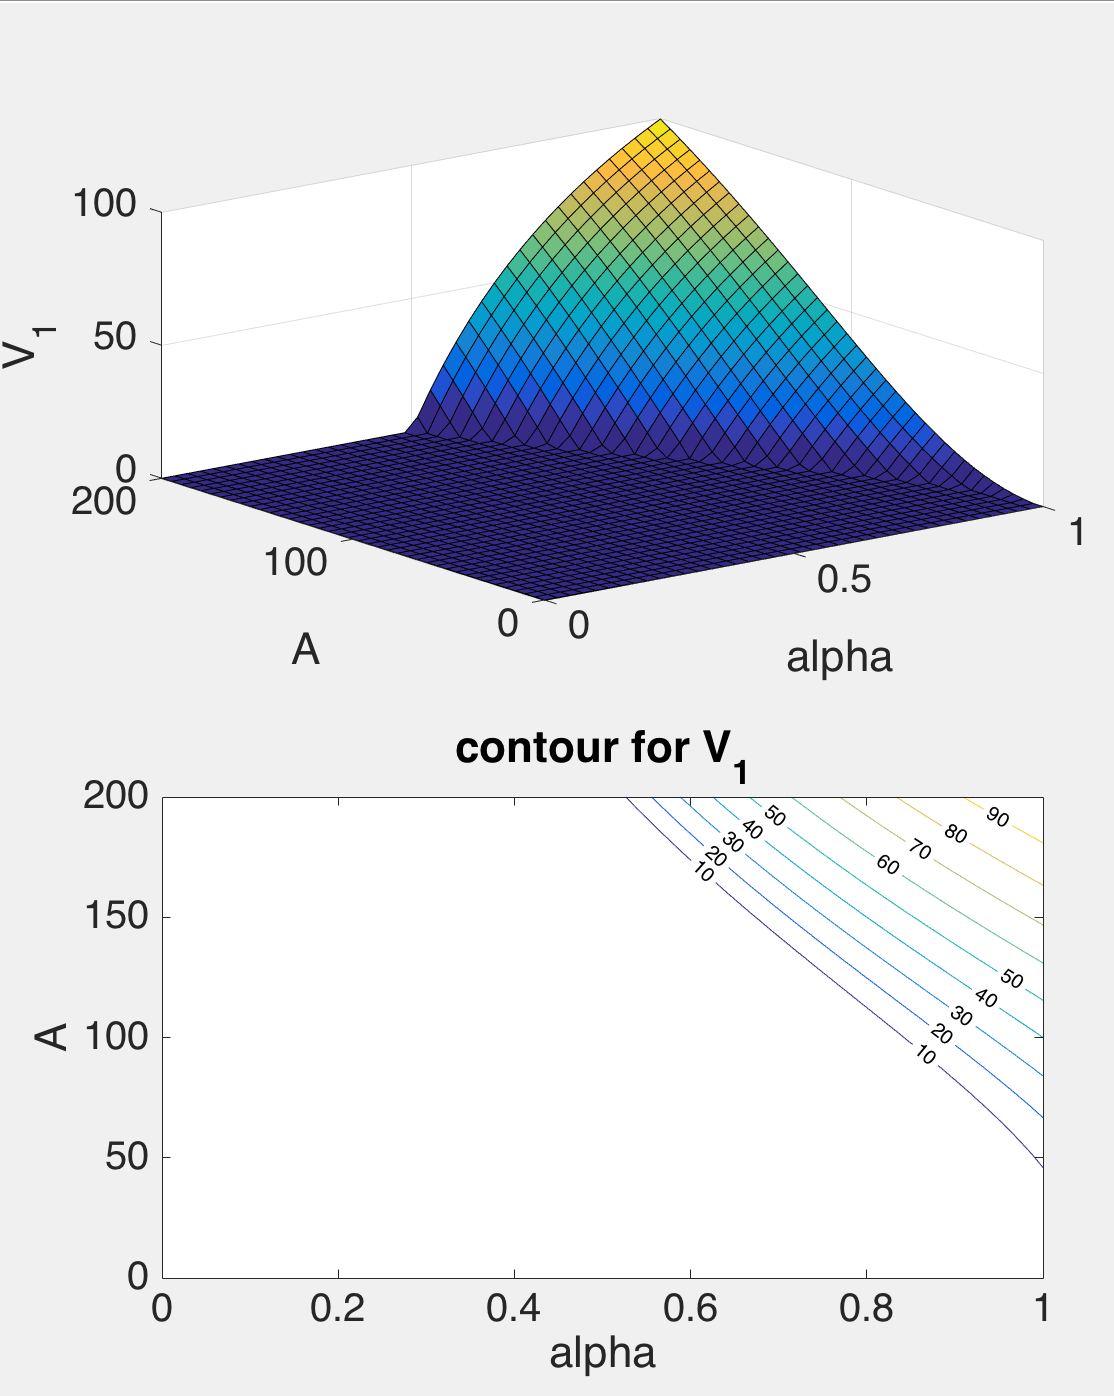
\includegraphics[width=200pt]{contourplot_basic}
\end{center}

Note that under specific settings of parameters as discussed above, it is possible for us to lose - left figure - or win - right figure (from Code Snippet 3). See the code for the parameter values used, and note that it follows the same relationship discussed.
\begin{center}
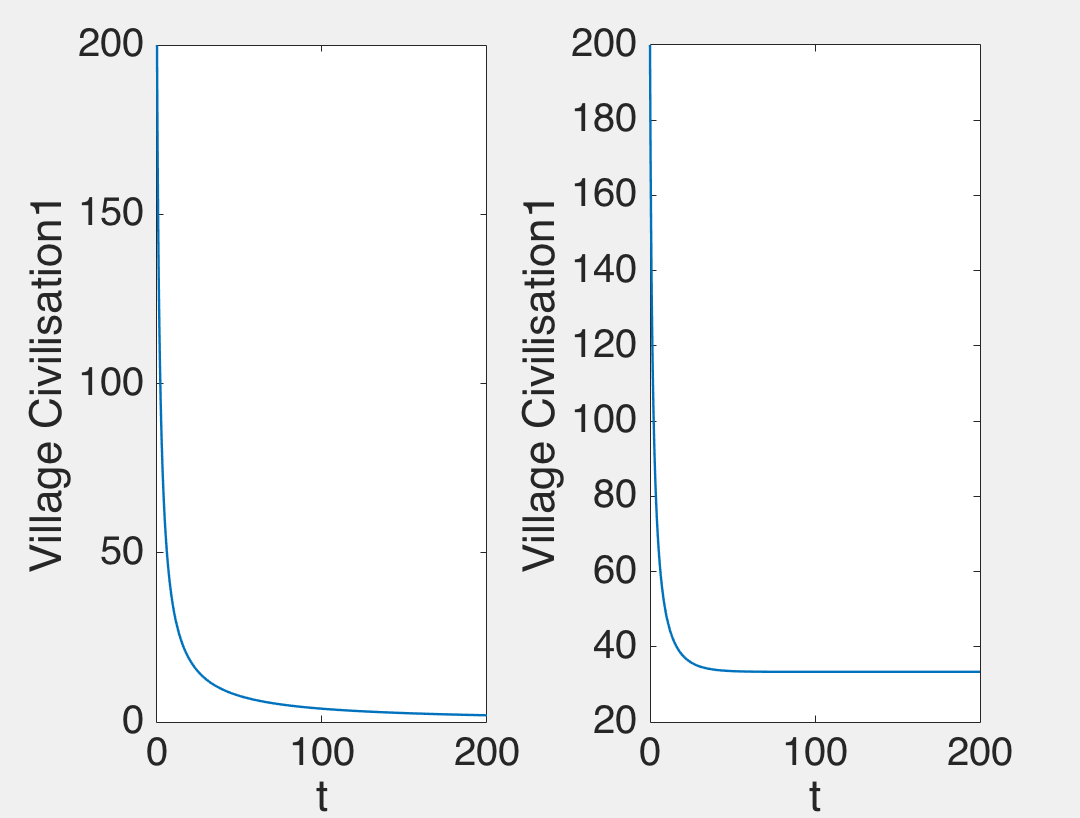
\includegraphics[width=200pt]{graph_basic}
\end{center}

\subsection{Scenario 2}
Here, because we have a system of ODEs, algebraic analysis is more difficult, but we can still perform some algebraic reasoning about the fixed points of the system. The equation for $\dot M_2$ implies that in the fixed point equilibrium $M_2 = 0$ or $M_1 = 0$ (or both are 0). If $M_1=0$, then $V_1=0$ or $V_1=(1-a)k$; if $V_1 = 0$, then $M_2$ can be anything (including 0) and if $V_1 = (1-a)k$, then $M_2$ must be 0. If $M_2 = 0$, then $V_1=0$ or $V_1=(1-a)k$; if $V_1 = 0$, then $M_1$ can be anything (including 0) and if $V_1 = (1-a)k$, then $M_1 = ak$. Because the only way to get $M_i = 0$ and $V_1 = (1-a)k$ is by setting $V_1(0) = (1-a)k$, we won't talk more about that fixed point. There are 3 remaining stable equilibrium scenarios from above:
\begin{enumerate}[(A)]
\item $V_1 = 0$, $M_1 = 0$, and $M_2 \geq 0$.
\item $V_1 =0$, $M_1 \geq 0$, and $M_2 = 0$.
\item $V_1 = (1-a)k$, $M_1 = ak$, and $M_2 = 0$.
\end{enumerate}

By changing the parameters $\alpha$, $A$, $a$, $D_1$, and $D_2$, we might vary the fixed point we reach. We can also do so with different initial conditions. Here are plots (from Code Snippet 4) that show the three different equilibrium scenarios - top left represents B, top right represents C, and bottom left represents A. Please see the code for the different parameter/ initial conditions settings that led to these varying equilibria:
\begin{center}
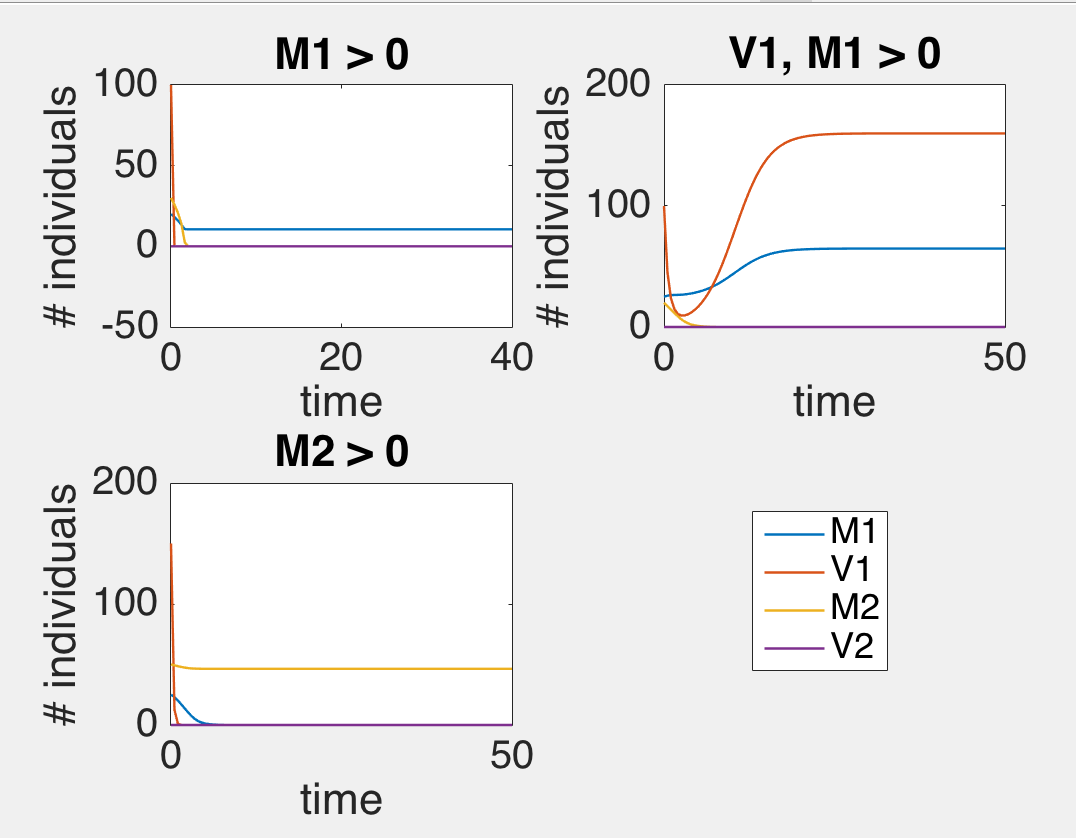
\includegraphics[width=200pt]{graph_ext1}
\end{center}

Now, let us consider how varying the parameters or initial conditions affects the equilibrium $M_1, V_1, and M_2$ solution - that is we will solve the ode numerically up to $t=40$ and read the value. We can consider two params at a time. In the first plot, let us consider $A$ and $\alpha$ as before (see Code Snippet 5). As you can see in the plot, holding other parameters constant, larger $A$ and $\alpha$ increase $M_1$ and $V_1$ repsectively for this solution. The behavior in the $M_2$ contour is just a byproduct of our ODE solver's imprecision.

\begin{center}
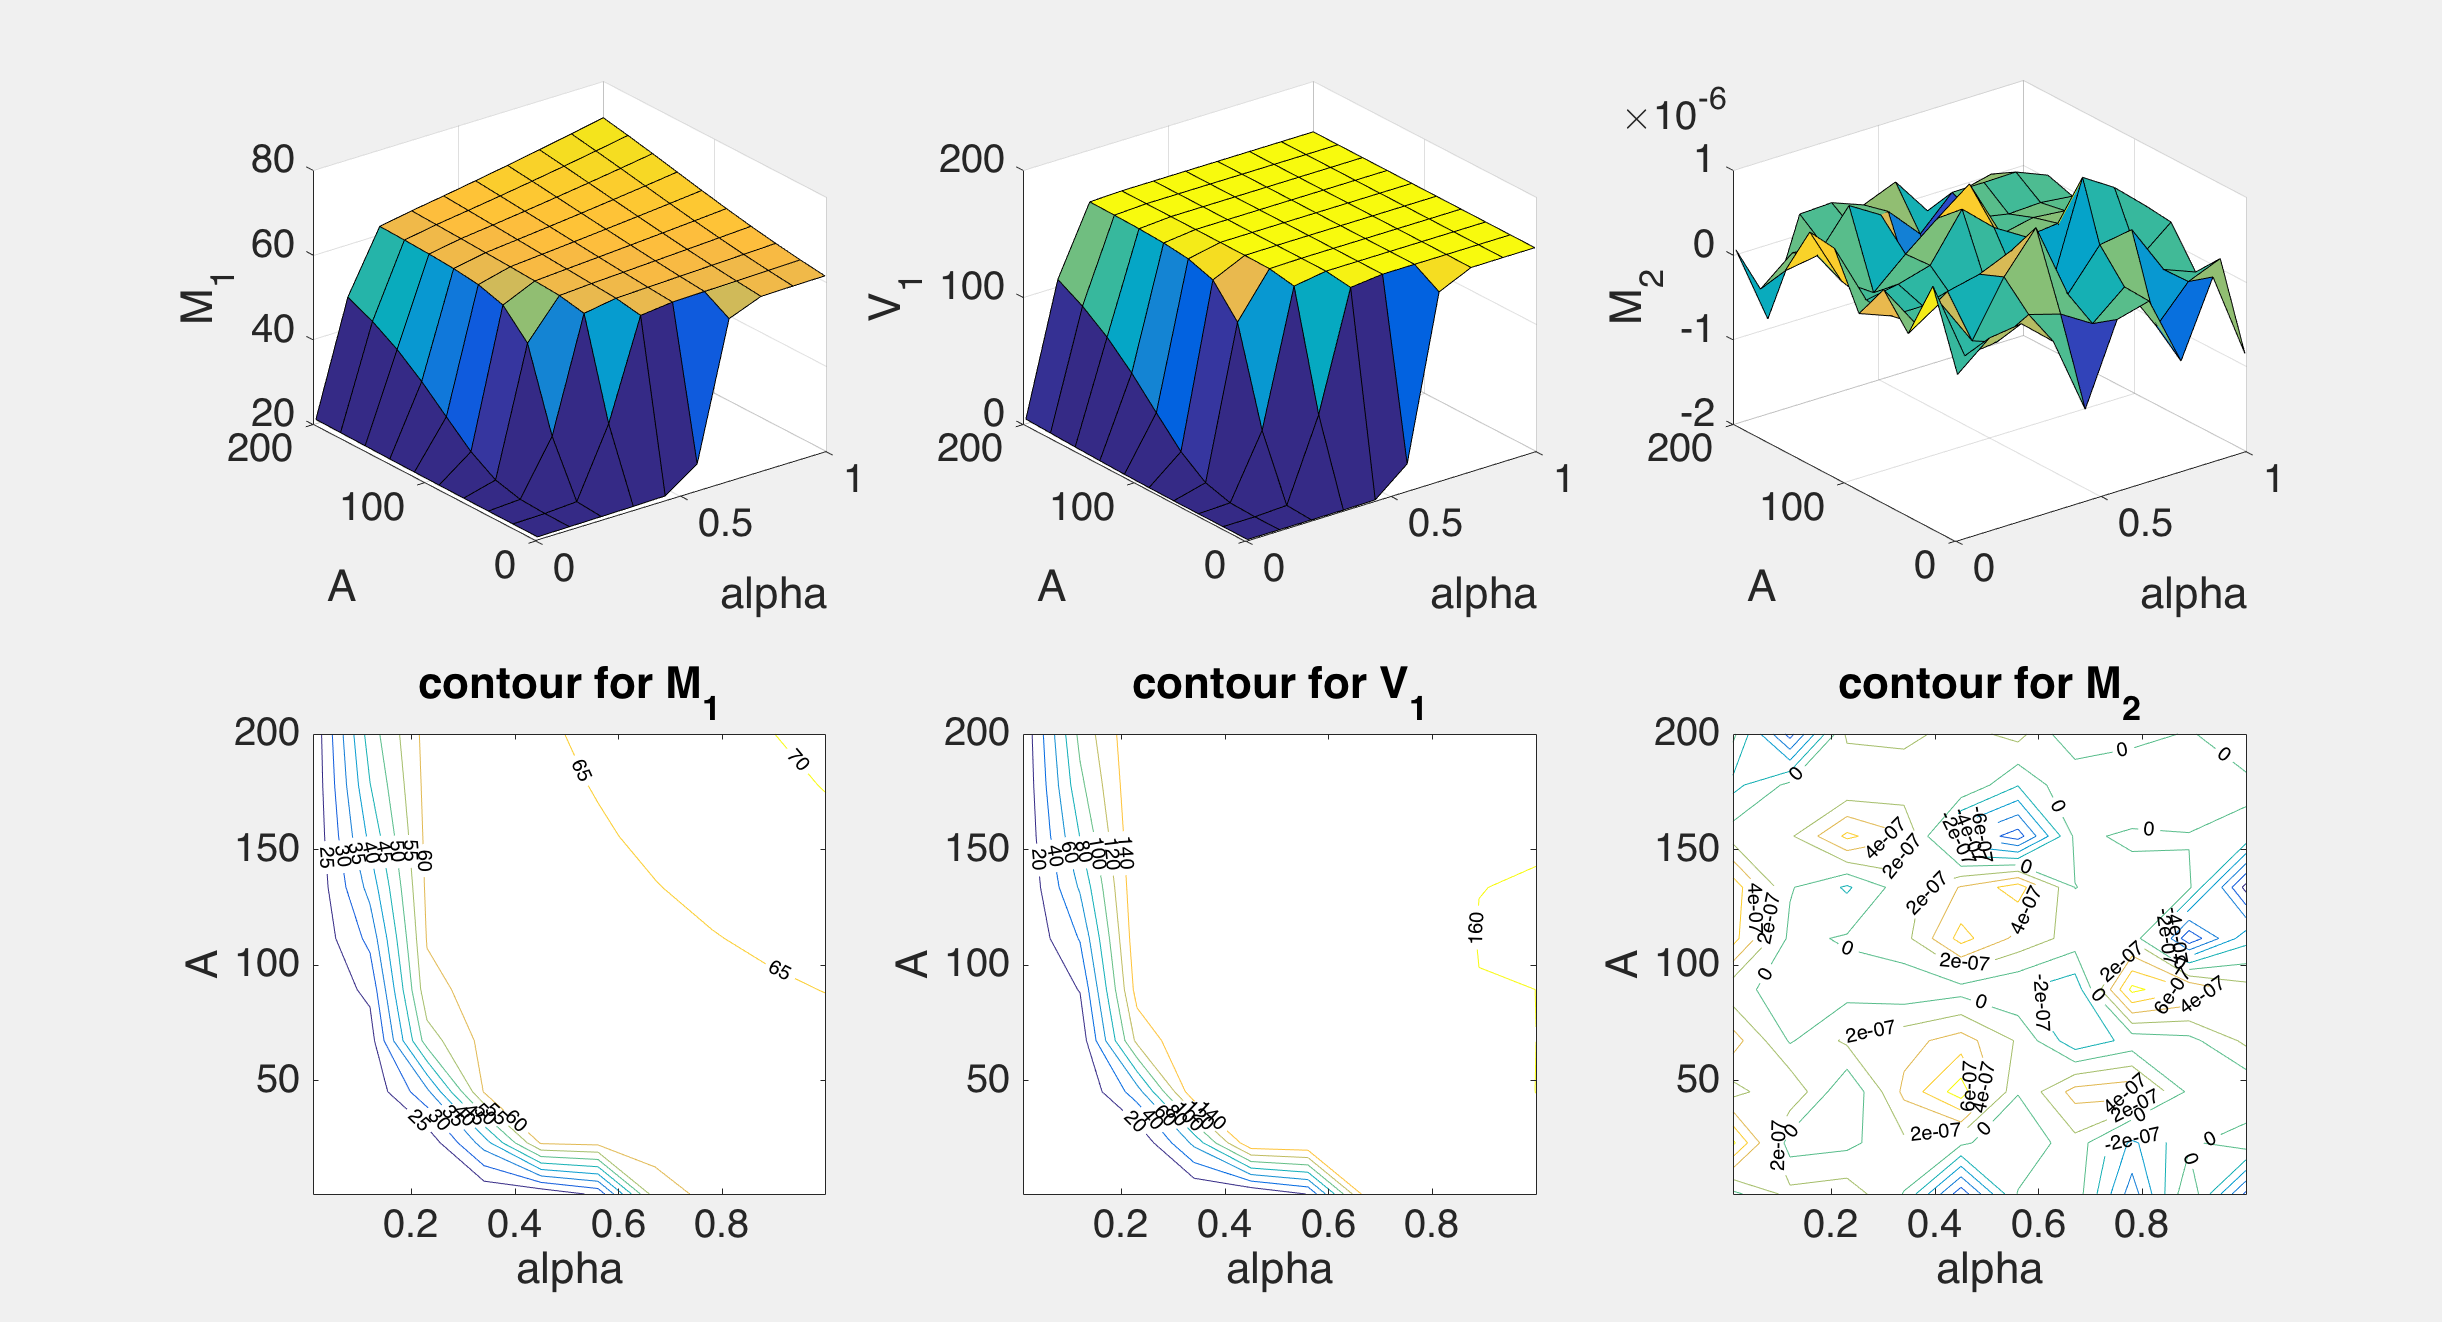
\includegraphics[width=300pt]{contour_ext1_part1}
\end{center}

In the next plot, we consider varying $D_1$ and $D_2$, which are the military effectiveness of $C_2$ and $C_1$ respectively (see Code Snippet 6). Let us consider the effect of varying these parameters with similar contour startegy as above. As you can see, small $D_1$ and high $D_2$ drive our populations of $M_1$ and $V_1$ to 0, and smaller $D_2$ can drive $V_1$ to 0 faster than $M_1$. As $D_1$ increases, $V_1$ increases, and as $D_2$ increases, $V_1$ decreases. For low $D_2$, as $D_1$ increases, $M_1$ generally decreases, and for high $D_2$, as $D_1$ increases, $M_1$ increases. As $D_2$ decreases, $M_1$ increases. Small $D_1$ and $D_2$ lead to high $M_1$ populations, when neither military is all that effective. Finally, higher $D_1$ leads to lower $M_2$ and higher $D_2$ leads to higher $M_2$. This is perhaps one of the more interesting interplay of parameters we will discuss in the Discussion section.

\begin{center}
\includegraphics[width=300pt]{contour_ext1_part2}
\end{center}

In the final plot, we observe the effects of varying initial conditions in an analagous fashion (see Code Snippet 7). Note that we will implicitly consider the parameter $a$ here, since $V_1(0) = \frac{1 - a}{a} M_1(0)$. We will consider initial conditions $M_1(0)$ versus $M_2(0)$. Here, as you can see, larger $M_1(0)$ increases $M_1$ and $V_1$ and decreases $M_2$. Similarly, larger $M_2(0)$ increases $M_2$ and decreases $M_1$ and $V_1$.

\begin{center}
\includegraphics[width=300pt]{contour_ext1_part3}
\end{center}


\subsection{Scenario 3}


\section{Discussion}
Before delving into contextualizing the results and further commenting on the behavior of models, let us briefly consider some limitations of our model. In the game, our allocations schedule might be more complicated than simply having the same proportion of villager and military births for all time, so this was a simplifying assumption we made. Furthermore, military units themselves can be split into archers, cavaliers, knights, etc. in the game, each of which have different properties and weaknesses/affinities towards one another in battle. Obviously, here too our model has made a simplifying assumption of uniformity in the types of miltary units. However, we can account for this somewhat in our model: if we have poor knowledge of the types of military units, then we can model this as a low $D_2$ parameter in our ODE because we will be less effective at killing the enemy AI.

\subsection{Scenario 1}
We found that in order to win, we needed $M_2^2 < \frac{\alpha}{1 - \alpha} A^2$, and we need to start with some villagers. This will allow us to reach a stable fixed point in which $V_1 > 0$ which will induce the enemy AI to surrender with enough time. This means if $M_2(0)$ is high like 200, we would need $\alpha > 0.5$ to win. If we set $\alpha = 1$, which means instantaneous spawn rates/ resource gathering, then regardless of map size, we should be able to sustain a non-zero population in the long run and thus win, which makes sense. If we choose a small map size (corresponds to low $A$ because it would be easier to find and kill villagers with even a small army), then we can also start the AI with a small military to win, or simply set a very high reproduction rate, i.e initialize a high unit spawn rate and gather resources quickly. \par

Thus, when initializing the game, we need to pick the right interplay of parameters between the military starting size of the AI, the map size, and the unit spawn rate, satisfying the above equation. Note that this will give us the best chance of winning, but not guarantee it, because if we are very slow at clicking villagers to resources in the actual gameplay, this will lower $\alpha$ and we may lose.  

\subsection{Scenario 2}
In this scenario, we can win by either destroying the military of the enemy AI, or sustaining population in the long run - equilibrium B and C from our analysis are victories, and equilibrium A is a loss. The initial conditions are parameters that we can set at game initialization (the amount of military the enemy AI starts with and the amount we start with), and the results we saw here aren't too surprising, i.e. that larger initial enemy military units hurt us, while as we have more initial military units, we have a higher chance of winning. \par
See scenario 1 discussion for thorough intuition on the parameters $A$ and $\alpha$. What we saw here was quite analagous - larger $A$ (think of it as map size) makes it hard for the enemy to find us, and larger $\alpha$ helps us maintain our populations (think of it as unit spawn rate). \par
Finally, let us contextualize the effects we observed that $D_1$ and $D_2$ had on the equilibrium quantities. $D_1$ can be thought of as the effectiveness of the enemy military while $D_2$ is the effectiveness of our military. In the game, we can influence $D_1$ through setting a difficulty level - at higher levels, the enemy is better able to use its military to maximize the number of your units it can kill. $D_2$ can be thought of as controlled by how fast we click and kill enemy units in the game; it can also be thought of as our "skill level" in the game. As we saw in the analysis, lower $D_1$ and higher $D_2$ is necessary to maximize our chances of winning. We must click quickly and strategize well, and we can set a lower difficulty at the start of the game to have a better chance of victory. We also saw from our contours that our villager population is driven to zero more quickly than our military, which suggests that we should initialize the game with many times more villagers to ensure that we can sustain populations. We also saw that for high $D_2$, increasing $D_1$ can actually increase $M_1$, but this just means that when we are incredibly effective at stifling the enemy military, increasing enemy military effectiveness doesn't hurt us as their populations are decreasing quickly anyway. We saw the surprising result that small $D_1$ and $D_2$ lead to incredibly high $M_1$ populations, but this is just because neither military is all that effective, so military units thrive. 
\subsection{Scenario 3}

\section{Conclusion} 
TODO: brief summary of motivation and discussion

\section{Attribution of Efforts} 
We attempted to keep it as fluid as possible, and came up with the model and helped each other on code through ~5 hours of meeting together. Nevertheless, here is rough split-up of work. Theresa wrote baseline code for scenario 1, began fixed point analysis, and wrote out the presentation pdf. Varun wrote the plots code for scenarios 2/3, extended the fixed points analysis, and put together most of the Latex File, collating results and tweaking (except Scenario 3). Steven came up with code for the contour plots, and added parts of Scenario 3 to the Latex File. Tina came up with the code for phase plots, and performed final organization/edits of the Latex File/Presentation, specifically adding portions to Scenario 3.

\section{References} 
\begin{enumerate}
\item \url{http://ageofempires.wikia.com/wiki/Age_of_Empires_III}
\item Class Notes from Zhiming Kuang
\end{enumerate}

\section{Code Appendix} 
\subsection{Snippet 1}
\begin{verbatim}
% Phase place plots of base case

clf; clear all

% Parameters, which can be varied to produce introducing results. 
alpha=0.5;
K=200; 
A=10;

% C_2=M_2= population of Civilization 2. Similarly, % C_1=V_1 = population
% of Civilization 1
% For this basic case, the population of Civ 2 is constant, since everyone
% is military and no one in Civ 1 is military, so Civ 2 cannot die
% Carrying capacity is 200, so we will make the phase portrait from 0 to
% 200
i=0;
for M_2=1:1:20
  i=i+1;
  j=0;
  for V_1=0:5:200
    j=j+1;
    VV1(i,j)=V_1;
    MM2(i,j)=M_2;
    dV_1(i,j)=alpha.*V_1.*(1-(V_1./K))-V_1*((M_2.^2)./(A^2+M_2.^2));
    dM_2(i,j)=0;
  end
end

% plot arrows in phase plane:
quiver(VV1,MM2,dV_1,dM_2)
h(1)=title('Civ 1 and Civ 2 populations');
h(2)=xlabel('Civilization 1');
h(3)=ylabel('Civilization 2');
h(4)=gca;
set(h,'FontSize',18)
axis([0 200 0 20])
hold on;


% plot fixed points - where the derivative is essentially 0 for both V_1
% and M_1
for i = 1:size(dM_2, 1)
    for j = 1:size(dV_1, 2)
        threshold = 0.3;
        if i == 9
            threshold = 0.1;
        elseif i == 10
            threshold = 0.01;
        elseif i == 3
            threshold = 1;
        elseif i == 1
            threshold = 0.6;
        end
        
        if abs(dV_1(i, j)) < threshold && abs(dM_2(i, j)) < threshold
            plot(VV1(i,j), MM2(i,j), 'r.', 'MarkerSize',20);
        end
    end
end
\end{verbatim}

\subsection{Snippet 2}
\begin{verbatim}
A_array = linspace(0, 200, 40);
alpha_array = linspace(0, 1, 40);

% Find fixed point vlaue for different A and alpha
for j=1:length(A_array)
    A = A_array(j);
    for k = 1:length(alpha_array)
        alpha = alpha_array(k);
        
        fixedpoint_V1(j, k) = basecase_v1_value(A, alpha, 200);
    end 
end

% in order to plot parameter dependencies
[X Y] = meshgrid(alpha_array, A_array);

subplot(2,1,1)
surf(X, Y, fixedpoint_V1)
xlabel('alpha')
ylabel('A')
zlabel('V_1')

subplot(2,1,2)
contour(X, Y, fixedpoint_V1, 'ShowText','on')
title('contour for V_1')
xlabel('alpha')
ylabel('A')

function V1 = basecase_v1_value(A, alpha, M20)
    % The fixed point calculation as decribed in the report
    stable_val = 200 * (1 - (1 / alpha) * (M20^2 / (A^2 + M20^2)));
    if stable_val < 0.5
        V1 = 0;
    else
        V1 = stable_val;
    end
end
\end{verbatim}

\subsection{Snippet 3}
\begin{verbatim}
function ode45_basic
clear all; close all;
M2=100;
V0=200;
K=200;
A=100;
B=100;
alpha=0.5;

[t,V1]=ode45(@(t,V1) f(t,V1,K,alpha,A,B, M2),[0 200],V0);
hold on;

subplot(1, 2, 1)
plot(t,V1)
xlabel('t');ylabel('Village Civilisation1')

alpha = 0.6;
[t,V1_new]=ode45(@(t,V1) f(t,V1,K,alpha,A,B, M2),[0 200],V0);

subplot(1, 2, 2)
plot(t,V1_new)
xlabel('t');ylabel('Village Civilisation1')


function ydot=f(t,V1,K,alpha,A,B, M2)
ydot=alpha*V1*(1-V1/K)-V1*M2^2/(A^2+M2^2);
\end{verbatim}

\subsection{Snippet 4}
\begin{verbatim}
clear all;

% This is when M1 > 0 and V1 and M2 are 0
[ t,P ] = solveExtension1(100,300, 8.17, 200, 1.0/6.0, 0.5, 20, 100, 30, 40);
subplot(2,2,1);
plot(t,P);
xlabel('time');
ylabel('# individuals');
title('M1 > 0');

clear all;

% This is when M1 > 0 and V1 > 0 and M2 = 0
[ a,b ] = solveExtension1(100,200,190, 200, 0.2, 0.5, 25, 100, 20, 50);
subplot(2,2,2);
plot(a,b);
xlabel('time');
ylabel('# individuals');
title('V1, M1 > 0');
legend('M1','V1','M2', 'V2');

clear all;

% This is when M2 > 0 and M1 and V1 equal 0
[ t,P ] = solveExtension1(200,100,190, 200, 1.0/7.0, 0.5, 25, 150, 50, 50);
subplot(2,2,3);
plot(t,P);
xlabel('time');
ylabel('# individuals');
title('M2 > 0');

% This is the function called by the above code
function [ t,P ] = solveExtension1(D1,D2,A, k, a, alpha, M10, V10, M20, tmax)

sol=ode45(@TwoCivmodel,[0 200],[M10,V10,M20,0]);

t=linspace(0,tmax);
P=deval(sol,t);

    function dP=TwoCivmodel(t,P)
        dP=zeros(4,1);     
        dP(1)=a*alpha*P(2)*(1 - P(2)/((1-a)*k)) - D1*P(1)*(P(3)^2 / (A + P(3)^2))*(1 / (A + P(1)^2));
        dP(2)=(1 - a)*alpha*P(2)*(1 - P(2)/((1-a)*k)) - 6*D1*P(2)*(P(3)^2 / (A + P(3)^2))*(1 / (A + P(1)));
        dP(3)= -D2*P(3)*(P(1)^2 / (A + P(1)^2))*(1 / (A + P(3)^2));
        dP(4)=0;
    end
end
\end{verbatim}

\subsection{Snippet 5}
\begin{verbatim}
clear all;

A_array = linspace(1, 200, 10);
alpha_array = linspace(0.01, 1, 10);

% Find M1, V1, M2 values for different A and alpha
for j=1:length(A_array)
    A = A_array(j);
    for k = 1:length(alpha_array)
        alpha = alpha_array(k);
        
	% see code snippet 4 for this function
        [ t,P ] = solveExtension1(100,200,A, 200, 0.2, alpha, 25, 100, 20, 50);
         
        M1(j, k) = P(1,100);
        V1(j, k) = P(2,100);
        M2(j, k) = P(3,100);
    end 
end

% in order to plot parameter dependencies
[X Y] = meshgrid(alpha_array, A_array);

subplot(2,3,1)
surf(X, Y, M1)
xlabel('alpha')
ylabel('A')
zlabel('M_1')

subplot(2,3,2)
surf(X, Y, V1)
xlabel('alpha')
ylabel('A')
zlabel('V_1')

subplot(2,3,3)
surf(X, Y, M2)
xlabel('alpha')
ylabel('A')
zlabel('M_2')


subplot(2,3,4)
contour(X, Y, M1, 'ShowText','on')
title('contour for M_1')
xlabel('alpha')
ylabel('A')

subplot(2,3,5)
contour(X, Y, V1, 'ShowText','on')
title('contour for V_1')
xlabel('alpha')
ylabel('A')

subplot(2,3,6)
contour(X, Y, M2, 'ShowText','on')
title('contour for M_2')
xlabel('alpha')
ylabel('A')

\end{verbatim}

\subsection{Snippet 6}
\begin{verbatim}
clear all;

D1_array = linspace(1, 200, 40);
D2_array = linspace(1, 200, 40);

% Find M1, V1, M2 values for different A and alpha
for j=1:length(D1_array)
    D1 = D1_array(j);
    for k = 1:length(D2_array)
        D2 = D2_array(k);
        
        % see code snippet 4 for this function
        [ t,P ] = solveExtension1(D1,D2,150, 200, 0.2, 0.5, 25, 100, 20, 50);
       
        M1(j, k) = P(1,100);
        V1(j, k) = P(2,100);
        M2(j, k) = P(3,100);
    end 
end

% in order to plot parameter dependencies
[X Y] = meshgrid(D1_array, D2_array);

subplot(2,3,1)
surf(X, Y, M1)
xlabel('D1')
ylabel('D2')
zlabel('M_1')

subplot(2,3,2)
surf(X, Y, V1)
xlabel('D1')
ylabel('D2')
zlabel('V_1')

subplot(2,3,3)
surf(X, Y, M2)
xlabel('D1')
ylabel('D2')
zlabel('M_2')


subplot(2,3,4)
contour(X, Y, M1, 'ShowText','on')
title('contour for M_1')
xlabel('D1')
ylabel('D2')

subplot(2,3,5)
contour(X, Y, V1, 'ShowText','on')
title('contour for V_1')
xlabel('D1')
ylabel('D2')

subplot(2,3,6)
contour(X, Y, M2, 'ShowText','on')
title('contour for M_2')
xlabel('D1')
ylabel('D2')

\end{verbatim}

\subsection{Snippet 7}
\begin{verbatim}
clear all;

M10_array = linspace(10, 200, 10);
M20_array = linspace(10, 200, 10);

% Find M1, V1, M2 values for different A and alpha
for j=1:length(M10_array)
    M10 = M10_array(j);
    for k = 1:length(M20_array)
        M20 = M20_array(k);
        
        disp(M10);
        disp(M20);
        % see code snippet 4 for this function
        [ t,P ] = solveExtension1(100,200,150, 200, 0.2, 0.5, M10, 4*M10, M20, 40);
      
        disp(P(1,100));
        
        M1(j, k) = P(1,100);
        V1(j, k) = P(2,100);
        M2(j, k) = P(3,100);
    end 
end

% in order to plot parameter dependencies
[X Y] = meshgrid(M10_array, M20_array);

subplot(2,3,1)
surf(X, Y, M1)
xlabel('M20')
ylabel('M10')
zlabel('M_1')

subplot(2,3,2)
surf(X, Y, V1)
xlabel('M20')
ylabel('M10')
zlabel('V_1')

subplot(2,3,3)
surf(X, Y, M2)
xlabel('M20')
ylabel('M10')
zlabel('M_2')


subplot(2,3,4)
contour(X, Y, M1, 'ShowText','on')
title('contour for M_1')
xlabel('M20')
ylabel('M10')

subplot(2,3,5)
contour(X, Y, V1, 'ShowText','on')
title('contour for V_1')
xlabel('M20')
ylabel('M10')

subplot(2,3,6)
contour(X, Y, M2, 'ShowText','on')
title('contour for M_2')
xlabel('M20')
ylabel('M10')

\end{verbatim}


\end{document}